\chapter{Hierarchical Clustering Background}
\label{cha:background2}

\section{Summary}
\label{sec:summary}

In this section we review the relevant terminology and background that is
required for the remainder of this thesis.  We begin with the general theory
of graphs, trees and their relationship to distances and special types of
metrics.  We then look at the problem of reconstructing trees from distances and
finally at the theory of ``lassoing'' a tree from incomplete distance
information.

\section{Graphs, Trees and Distances}
\label{sec:graphs-trees-dist}

\subsection{History}
\label{sec:history}

Trees have been used to represent hierarchical structures for many hundreds of
years \cite{knuth97taocp1}.  One of the most well-known and ubiquitous
occurrences is that of the family tree.  The use of a tree to represent
lineages was widespread in Europe by the 14th Century in Christian artwork
depicting the ancestors of Jesus of Nazareth.  This depiction is known as the
Tree of Jesse \cite{corblet1860etude}.

Darwin would later popularise the concept of the more general ``tree of life''
in his seminal work popularly known as \textit{On the Origin of Species}
\cite{darwin1859origin}.  Darwin's first tree (Figure~\ref{fig:darwin-tree})
shows the theoretical relationship between an ancestral species (1) and its
descendant species \cite{semple2003phylogenetics}.  Extant species are shown
by tips on the endpoints of some branches with the remaining branches possibly
representing extinct species.  His idea was that groups of species would have
diverged at different times and therefore some groups will be more closely
related than others.  For example, the species labelled by B and C would be
more closely related than those labelled by A and D.

\begin{figure}
  \centering
  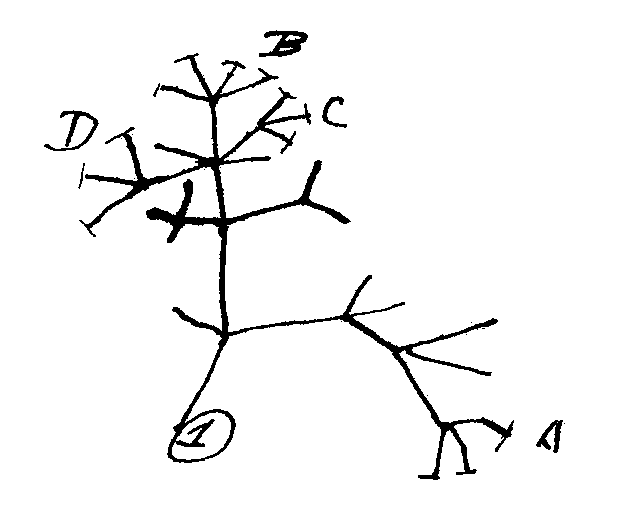
\includegraphics[width=20em]{figures/background2/darwin-tree.png}
  \caption{Charles Darwin's first diagram of an evolutionary tree from his
    notebook \textit{Transmutation of species}, 1837 \cite{darwin1837notebook}.}
  \label{fig:darwin-tree}
\end{figure}

Trees as a formally defined mathematical entity, such as the ones will see in
the following sections, appeared as early as 1847 with the name ``tree''
appearing in the literature shortly afterwards \cite{knuth97taocp1}.  The more
general theory of graphs and topology was developed earlier and is considered
to have begun with Euler who in 1735 presented the paper ``Solutio problematis
ad geometriam situs pertinentis'' \cite{euler1735solutio} in which it was
shown that it was not possible to walk through the city of Königsburg crossing
each of its seven bridges exactly once.

Tree structures are of great importance in computer programming.  One of the
earliest programs to make explicit use of tree structures used them to
represent algebraic formulae for the purpose of symbolic differentiation
\cite{knuth97taocp1,kahrimanian53differentiation}.  This would later become
the field of computer algebra which would drive the development of computer
science and especially programming languages for many years.

Intuitively, it makes sense to arrange many different types of information in
trees, particularly that for which we can define a distance since.  A first
question to ask is whether a representation in terms of a tree exists for a
given dataset and distance function.  As we will see, when the distance
function satisfies certain properties there always exists a tree
representation and this representation is also unique (in a well-defined
sense).  We focus then on a slightly different problem: imagine we know the
distance between only certain pairs of objects in our dataset.  We call this
information a partial distance.  This presents two separate problems.  First,
does there exist a tree representation of a given partial distance and if so,
can we find one?  Second, does there exist a unique tree representation of a
given partial distance, and if so can we find it?  These issues are the
subject of the remainder of this thesis.

\subsection{Basic terminology and assumptions}
\label{sec:basic-term-assumpt}

In this section we introduce much of the terminology that is required for
dealing with trees.  Since trees are special cases of graphs, we begin with
general graph theory before moving on to trees and, in particular, a special
type of tree that is of greatest interest to us: the equidistant tree.  As
noted by Knuth \cite{knuth97taocp1} there is a large degree of variation in
the terminology used by different authors in graph theory.  We try to follow
the terminology used in current phylogenetics literature such as
\cite{semple2003phylogenetics} and \cite{dress11lassoing}.  Throughout this
section, let $X$ denote a finite nonempty set.

\subsubsection{Graphs}
\label{sec:graphs}

A \textit{graph} is an ordered pair $(V,E)$ where $V$ is a set of
\textit{vertices} and $E$ is a set (or multiset) of \textit{edges}, each of
the form $\{x,y\}$ such that $x,y \in V$ are distinct.  Unless specified
otherwise, all graphs in this thesis are \textit{simple} and finite meaning
that $V$ and $E$ are finite sets and there are no loops.  Suppose $G = (V,E)$
is a graph. Two vertices $v,v' \in V$ are said to be \textit{adjacent} if
there exists an edge in $G$ joining $v$ and $v'$.  An edge $\{x,y\} \in E$ is
said to be \textit{incident} with the vertices $x$ and $y$.  The
\textit{degree} of a vertex $v \in V$ is the number of edges in $G$ incident
with it.

\begin{figure}
  \centering
  \input{figures/background2/graph-ex.pdft}
  \caption{A graph (i) and a directed graph (ii).}
  \label{fig:graph-ex}
\end{figure}

A \textit{path} is a sequence of distinct vertices $v_1,v_2,\dotsc,v_k$ where
$k \geq 2$ such that for all $i \in \{1,\dotsc,k-1\}, v_i$ and $v_{i+1}$ are
adjacent.  If $k \geq 3$ and $v_1$ and $v_k$ are also adjacent then the path
is called a \textit{cycle}.  A graph is \textit{connected} if between each
pair of distinct vertices there exists a path joining them.  A graph is
\textit{complete} if there is an edge joining each pair of distinct vertices.
A subset $V' \subseteq V$ is called a \textit{clique} if there is an edge
joining each pair of distinct vertices in $V'$.  Figure~\ref{fig:graph-ex}
helps to illustrate these definitions.  In the graph shown in (i) an example
of a path is $g,f,e,d$ and an example of a cycle is $g,f,b,a,g$.  The graph is
connected, but not complete, and the set $\{a,b,g,f\}$ is a clique.

A \textit{directed graph} is an ordered pair $(V,E)$ where $E$ is a set of
\textit{directed edges} or \textit{arcs}.  An arc $(v,v') \in E$ is said to
lead from $v$ to $v'$.  The \textit{out-degree} of a vertex is the number of
arcs leading out from it and the \textit{in-degree} is the number leading in.
The degree of a vertex is therefore the sum of its out-degree and in-degree.
An \textit{oriented path} is a sequence of distinct vertices $v_1,\dotsc,v_k$
such that there exists an arc from $v_i$ to $v_j$ for all $1 \leq i \leq k-1$.
Figure~\ref{fig:graph-ex} (ii) shows a directed graph to help illustrate these
definitions.  Vertex $f$ has out-degree 3, in-degree 1 and therefore degree 4.
An example of an oriented path is $e,f,b,c$.

Two graphs $(V,E)$ and $(V',E')$ are called \textit{isomorphic} if there
exists a bijection $\phi \colon V \to V'$ such that $\{v,v'\} \in E$ if and
only if $\{\phi(v),\phi(v')\} \in E'$.  So, in other words, adjacency of
vertices is preserved.  A graph $(V',E')$ is a \textit{subgraph} of a graph
$(V,E)$ if $V' \subseteq V$ and $E' \subseteq E$.  Further if $V' \subseteq V$
and $E'$ contains all edges $\{v,v'\} \in E$ whenever $v,v' \in V'$ the graph
$(V',E')$ is an \textit{induced subgraph} of $(V,E)$.

\subsubsection{Trees}
\label{sec:trees}

In this section we formally define trees as a special type of graph and
introduce all the relevant terminology for a special type of tree which we
will focus on.

A graph that is connected and has no cycles is called a
\textit{tree}.  Trees can be characterised in many ways, some of which are
given in the following theorem (see \cite[][Section 2.3.4.1]{knuth97taocp1}
for a proof):

\begin{thm}
  If $G$ is a finite graph with $n > 0$ vertices, the following statements are
  equivalent:
  \begin{enumerate}[label=\alph*)]
  \item $G$ is a tree,
  \item $G$ is connected, but if any edge is deleted the resulting graph is no
    longer connected,
  \item There is exactly one path between any two distinct vertices of $G$,
  \item $G$ contains no cycles and has $n-1$ edges,
  \item $G$ is connected and has $n-1$ edges.
  \end{enumerate}
\end{thm}

For example, Figure~\ref{fig:x-tree-ex} shows two graphs which are trees.  The
tree depicted in (ii) is a special type of tree called a \textit{rooted tree}.
A rooted tree (or \textit{oriented tree}) is a directed graph $G$ with a
distinguished vertex $\rho_G$ (the root) such that \cite{knuth97taocp1}:
\begin{enumerate}[label=\alph*)]
\item The root $\rho_G$ has in-degree 0,
\item Each vertex $v$ of $G$ apart from $\rho_G$ has in-degree 1,
\item There is a path between $\rho_G$ and any vertex of $G$ that is not the
  root.
\end{enumerate}

\begin{figure}
  \centering
  \input{figures/background2/x-tree-ex.pdft}
  \caption{A tree (i) and a rooted phylogenetic $X$-tree
    (ii).}
  \label{fig:x-tree-ex}
\end{figure}

Suppose $T$ is a rooted tree.  A vertex in $T$ is called a \textit{leaf} if it
has degree 1.  All other vertices are called \textit{interior} vertices.  An
edge which is incident with a leaf is called a \textit{pendant} edge.  All
other edges are called \textit{interior} edges.  The set of all leaves of $T$
is called the \textit{leafset} of $T$ which we denote by $L(T)$.

Suppose $X$ is a finite, nonempty set, a \textit{rooted phylogenetic $X$-tree}
is a rooted tree with no vertices of in-degree one and out-degree one and with
leafset $X$.  Since the remainder of this thesis is concerned with rooted
trees we will from now on refer to a rooted phylogenetic $X$-tree as simply an
\textit{$X$-tree}.  Figure~\ref{fig:x-tree-ex} (ii) shows an $X$-tree with $X
= \{a,\dotsc,f\}$.

An $X$-tree is \textit{binary} if all interior vertices have degree 3 apart
from the root which has degree 2.  We therefore have that each vertex has
out-degree zero or two and each vertex apart from the root has in-degree 1.
By considering the directed paths from the root to leaves it becomes clear why
such a tree is called binary \cite{semple2003phylogenetics}.

An \textit{edge-weighted graph} $(G,\omega)$ is a graph $G=(V,E)$ paired with
an edge-weighting function $\omega \colon E \to \rr$.  For an edge-weighted
$X$-tree $T$ we call an edge-weighting \textit{proper} if $w(e) > 0$ for every
interior edge $e$ of $T$.

An $X$-tree has a natural partial order on the vertices.  Given an $X$-tree
$T=(V,E)$, a vertex $v \in V$ is an \textit{ancestor} of a vertex $v' \in V$
if and only if $v$ is on the directed path from the root of $T$ to $v'$.  The
vertex $v'$ is then said to be a \textit{descendant} of $v$.  If $v$ and $v'$
are adjacent then we also call $v$ the \textit{parent} of $v'$ and $v'$ a
\textit{child} of $v$.  The number of children of a particular vertex equals
its out-degree.

The \textit{lowest common ancestor} of two vertices $v$ and $v'$ in an
$X$-tree is the unique vertex $u$ such that $u$ is an ancestor of both $v$ and
$v'$ and the path from the root $\rho$ to $u$ is longer than the path to any
other ancestor of both $v$ and $v'$.  The lowest common ancestor of $v$ and
$v'$ is denoted $\lca(v,v')$.  In the $X'$-tree in Figure~\ref{fig:x-tree-ex}
(ii) the lowest common ancestor of $a$ and $d$ is the root $\rho$.

A connected subgraph of a tree is called a \textit{subtree}.  If $T$ is an
$X$-tree and $X' \subseteq X$ then we denote by $T|X'$ the subtree of $T$
whose leafset is $X'$, with degree 2 vertices suppressed.  $T|X'$ is then
called a \textit{restricted subtree}.  If $T$ is binary and $|X'| = 3$ then
$T|X'$ is called a \textit{triplet}.

We call two $X$-trees $T$ and $T'$ \textit{equivalent} (written $T \simeq T'$)
if there exists a bijection $\phi \colon V(T) \to V(T')$ that extends to a
graph isomorphism that is the identity on $X$.  Since an $X$-tree is rooted,
$\phi$ must also map $\rho_{T}$ to $\rho_{T'}$.

For a set $X$ the number of possible non-equivalent binary $X$-trees is
$(2|X|-3)!!$.  Therefore to find a tree in this space with particular
properties we cannot look at each possible tree and must instead use a special
tree reconstruction method.  Next we look at how distances are related to
trees and then at the problem of reconstructing a tree from distance
information.

\subsubsection{Ultrametrics}
\label{sec:ultrametrics}

Given an edge-weighted $X$-tree $(T,\omega)$ where $T=(V,E)$ and $\omega
\colon E \to \rrnn$ we can associate a distance $D_{(T,\omega)} \colon X
\times X \to \rrnn$ to $(T,\omega)$ by setting for all $x,y \in X$:
\begin{equation*}
  D_{(T,\omega)}(x,y) =
  \begin{cases}
    \displaystyle
    \sum_{e \in P(x,y)} \omega(e) & \text{if $x \neq y$},\\
    0 & \text{otherwise,}
  \end{cases}
\end{equation*}
where $P(x,y)$ is the set of edges on the path from $x$ to $y$.  We call
$D_{(T,\omega)}$ the distance \textit{induced} by $(T,\omega)$.  

The distance induced by a tree is a special type of metric called a
\textit{tree metric}.  These metrics have some interesting properties which
are discussed in \cite[Chapter 7]{semple2003phylogenetics}.  For our purposes
we are most interested in a special type of tree metric called an
\textit{ultrametric}.  A distance $\delta \colon X \times X \to \rr$ is called
an ultrametric if for every distinct $x,y,z \in X$ the following stronger form
of the triangle inequality holds:
\begin{equation*}
  \delta(x,y) \leq \max(\delta(x,z),\delta(y,z)).
\end{equation*}

\begin{figure}
  \centering
    \begin{subfigure}[b]{0.5\textwidth}
      \centering
      \input{figures/background2/treeconstruct1.pdft}
      \label{fig:example-equidistant-1}
      \caption{}
    \end{subfigure}%
    ~
  \begin{subfigure}[b]{0.5\textwidth}
    \centering
    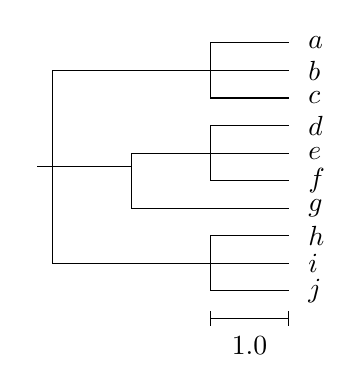
\begin{tikzpicture}[yscale=0.35]
    \node (r) at (0.0,0.0) {};
\node (rr) at (-0.2,0.0) {};
\draw (r.center) -- (rr.center);
\node (r1) at (2.0,-3.5) {};
\node[label=right:{$j$}] (r11) at (3.0,-4.5) {};
\draw (r1.center) |- (r11.center);
\node[label=right:{$i$}] (r12) at (3.0,-3.5) {};
\draw (r1.center) |- (r12.center);
\node[label=right:{$h$}] (r13) at (3.0,-2.5) {};
\draw (r1.center) |- (r13.center);
\draw (r.center) |- (r1.center);
\node (r2) at (1.0,0.0) {};
\node[label=right:{$g$}] (r21) at (3.0,-1.5) {};
\draw (r2.center) |- (r21.center);
\node (r22) at (2.0,0.5) {};
\node[label=right:{$f$}] (r221) at (3.0,-0.5) {};
\draw (r22.center) |- (r221.center);
\node[label=right:{$e$}] (r222) at (3.0,0.5) {};
\draw (r22.center) |- (r222.center);
\node[label=right:{$d$}] (r223) at (3.0,1.5) {};
\draw (r22.center) |- (r223.center);
\draw (r2.center) |- (r22.center);
\draw (r.center) |- (r2.center);
\node (r3) at (2.0,3.5) {};
\node[label=right:{$c$}] (r31) at (3.0,2.5) {};
\draw (r3.center) |- (r31.center);
\node[label=right:{$b$}] (r32) at (3.0,3.5) {};
\draw (r3.center) |- (r32.center);
\node[label=right:{$a$}] (r33) at (3.0,4.5) {};
\draw (r3.center) |- (r33.center);
\draw (r.center) |- (r3.center);
\draw[|-|] (2.0,-5.5) -- (3.0,-5.5);
\node at (2.5,-6.5) {1.0};
     \end{tikzpicture}
     \caption{}
     \label{fig:example-equidistant-2}
   \end{subfigure}

   \caption{A dendrogram is a visual representation of a tree.  Here we see
     two different ways to draw the same edge-weighted $X$-tree.}
   \label{fig:example-equidistant}
\end{figure}

An edge-weighting $\omega \colon E \to \rr$ for an $X$-tree $T=(V,E)$ with
root $\rho_T$ is called \textit{equidistant} if it satisfies the following
properties:
\begin{itemize}
\item[(i)] $D_{(T,\omega)}(\rho_T,x) = D_{(T,\omega)}(\rho_T,y)$ for all $x,y
  \in X$,
\item[(ii)] $D_{(T,\omega)}(x,y) \geq D_{(T,\omega)}(x,u)$ for all $x \in X$
  and any $u,v \in V$ whenever $u$ is encountered before $v$ on the directed
  path from $x$ to $\rho$.
\end{itemize}
If $\omega$ is an equidistant edge-weighting then $D_{(T,w)}$ is an
ultrametric \cite[Lemma 7.2.4]{semple2003phylogenetics}.  $X$-trees with
equidistant edge-weightings arise naturally in many places, for example in
phylogenetics.  For convenience we will from now on refer to such an $X$-tree
with equidistant edge-weighting as simply an \textit{equidistant $X$-tree}.

Figure~\ref{fig:example-equidistant} shows an example of an equidistant
$X$-tree with $X = \{a, \dotsc, j\}$ using two common display formats
(dendrograms).  In (i) the edges are simply labelled with their weights (edges
with weight 1 are left unlabelled for clarity).  In (ii) the weight of each
edge is proportional to the horizontal component of its length on the bar with
the actual length shown with a scale bar.

For any ultrametric $\delta \colon X \times X \to \rr$ there is, up to
isomorphism, a unique equidistant $X$-tree $(T,\omega)$ such that $\delta(x,y)
= D_{(T,\omega)}(x,y)$ for all $x,y \in X$.  This tree can be recovered from
the ultrametric in polynomial time, as we will see in the next section.

\section{Tree reconstruction}
\label{sec:tree-construction}

In this section, we look at various methods of reconstructing trees.  Of most
interest to us is the problem of reconstructing an $X$-tree from a distance on
$X$.  This is generally done by one of two broad classes of hierarchical
clustering methods which we discuss in Section~\ref{sec:hier-clust-meth}.

A further problem is that of reconstructing an edge-weighted $X$-tree from a
distance on $X$.  This is desirable in many cases, for example in
phylogenetics the edge-weights might represent the time or number of point
mutations \cite{felsenstein2004inferring}.

Closely related to this is the problem of reconstructing $X$-trees from only
partial distance information.  This means that we do not have the complete
distance $d$, but rather only have the values $d(x,y)$ for some, but not all,
pairs $x,y \in X$.  This problem is motivated by the fact that accurate
distance measurements are often difficult or impossible to obtain in practice
but one would still like to build an edge-weighted $X$-tree given only what is
known.

As with complete distance information, it is possible for partial distance
information to uniquely determine an $X$-tree.  This is the subject of
Section~\ref{sec:lassoing-corralling}.  This allows us to define a consistency
property for partial distance reconstruction methods.

\subsection{Reconstruction from subtrees}
\label{sec:constr-from-subtr}

Before we look at reconstructing trees from distances, it is interesting to
note that we do not actually need a distance to reconstruct only the topology
of an $X$-tree.  It suffices merely to know the set of subtrees displayed by
the tree \cite{semple2003phylogenetics}.

A pair of leaves of an $X$-tree that share the same parent is called a
\textit{cherry} and a set of leaves (of any size) that share the same parent
is called a \textit{pseudocherry}.  As before, an $X$-tree with $|X| = 3$ that
contains a cherry is called a triplet.  If $P$ is an $\{a,b,c\}$-tree $a,b$ is
a cherry of $P$ then we denote the triplet $P$ by $ab|c$.  We say that a
triplet $ab|c$ is \textit{displayed} by an $X$-tree $T$ if the restriction
$T|\{a,b,c\}$ of $T$ to $\{a,b,c\}$ is binary and $lca_T(a,c) = lca_T(b,c)$ is
an ancestor of $lca_T(a,b)$ in $T$.  For example, the tree $T_2$ in
Figure~\ref{fig:build-ex} is a triplet and can be written as $ad|c$.

\begin{algorithm}[h]
  \caption{\textsc{Build}.}
  \label{alg:build}

  \begin{algorithmic}
    \Require A set of rooted trees $R = \{T_1,\dotsc,T_n\}$.
    \Ensure  An $X$-tree $T$ where $X = L(T_1) \cup \dotsb \cup L(T_n)$.

    \State $S = \{x_1,\dotsc,x_m\} \gets X$.

    \If{$|S| = 1$} \Return the tree $(\{x_1\},\emptyset)$. \EndIf

    \If{$|S| = 2$} let $\rho$ be a new vertex and \Return the tree with root
    node $\rho$ obtained by attaching $x_1$ and $x_2$ to $\rho$. \EndIf

    \State Construct the auxiliary graph $[R,S]$.

    \State Let $S_1,\dotsc,S_k$ be the vertex sets of the connected components
    of $[R,S]$.

    \ForAll{$1 \leq i \leq k$}
    \State Let $T_i$ be the output of \textsc{Build} on $R_i =
    \{T|S_i \colon T \in R\}$.
    \EndFor

    \State Let $\rho$ be a new vertex and \Return the tree with root node
    $\rho$ obtained by attaching the root of each $T_i$ to $\rho$.
    
  \end{algorithmic}
\end{algorithm}

\begin{figure}
  \centering
  \input{figures/background2/build-ex2.pdft}
  \caption{An illustration of \textsc{Build} with an input of $R =
    \{T_1,T_2\}$.  $[R,S]$ is the auxiliary graph built in the first iteration
    of the algorithm and $T$ is the final tree constructed.}
  \label{fig:build-ex}
\end{figure}

The \textsc{Build} algorithm \cite{aho1981inferring} can be used to
reconstruct an $X$-tree $T$ from the set of all triplets displayed by $T$.  We
show the \textsc{Build} algorithm in pseudocode in Algorithm~\ref{alg:build}
and give an example in Figure~\ref{fig:build-ex}.  The algorithm uses a set
$R$ of rooted trees $\{T_1,\dotsc,T_n\}$ where $L(T_1) \cup \dotsb \cup L(T_n)
= X$ and an auxiliary graph $[R,S]$ which has vertex set $S \subseteq X$ and
an edge $\{a,b\}$ for each $a,b \in S$ whenever there exists some $c \in S$
and some $T' \in R$ such that $T'|\{a,b,c\}$ and $ab|c$ are equivalent.

This algorithm has some nice properties, for example if \textsc{Build} returns
a tree then the set of input trees is said to be \textit{compatible}.  The
definition of compatible is independent of \textsc{Build} (see
\cite{semple2003phylogenetics}) but \textsc{Build} can be used to check
compatibility.  Furthermore, if we input the set of all triplets displayed by
a tree $T$, then \textsc{Build} is guaranteed to output $T$ and therefore $T$
is uniquely determined by the set of triplets it displays.

If the inputted set of triplets $R$ is some subset of all the triplets
displayed by a tree then the set is still compatible but this set is displayed
by possibly many trees.  In this case the output of \textsc{Build} is
deterministic and the tree reconstructed is known as \textit{the
  \textsc{Build} tree for $R$}.  Some interesting properties of these trees
can be found in \cite[Section 2.5.2]{bryant97buildingtrees}.

The \textsc{Build} algorithm was initially developed to construct a tree
satisfying a given set of constraints and was applied to problems arising in
the theory of relational databases.  It was later applied to phylogenetics but
remained relatively unknown in the field for a number of years
\cite{steel1992complexity,bryant04supertree}.

When the inputted trees are not compatible, \textsc{Build} returns an error.
Since it is often the case that trees will not be compatible, the
\textsc{MinCutSupertree} algorithm was developed which will construct a tree
even if the input trees are not compatible \cite{semple2000supertree}.
The algorithm builds a graph similar to $[R,S]$ and ensures that it is
disconnected in each step by using a minimum cut.  This algorithm was
developed primarily for construction of phylogenetic supertrees.

\subsection{Reconstruction from distances}
\label{sec:constr-from-dist}

We now turn to the problem of reconstructing an $X$-tree from a distance.  We
begin with a brief overview of general hierarchical clustering methods and
then look at the UPGMA method \cite{sokal1958statistical} and its optimal
runtime algorithm.  Hierarchical clustering methods in general build
unweighted $X$-trees, but UPGMA can be considered an extension which also
constructs an edge-weighting for the constructed tree.

For a distance-based reconstruction method the following property is
desirable: if we input a distance function $D_{(T,\omega)}$ induced by an
edge-weighted $X$-tree $(T,\omega)$ we get the tree $T$ and its edge-weighting
$\omega$.  If a method enjoys this property then we call it
\textit{consistent}.  For many methods this property holds only under certain
conditions.  For UPGMA this holds if $(T,\omega)$ is a binary equidistant
$X$-tree \cite{durbin1998biological}.

\subsubsection{Hierarchical clustering methods}
\label{sec:hier-clust-meth}

\begin{figure}
  \centering
  \input{figures/background2/tree-clust-ex.pdft}
  \caption{A tree can be viewed as a hierarchy of partitions.}
  \label{fig:tree-clust-ex}
\end{figure}

Hierarchical clustering is used for the classification of information in much
the same way as partitional clustering.  The aim of a hierarchical clustering
method is to produce an $X$-tree corresponding to a given distance $D$ on a
set $X$.  While a partition of a set is merely a set of disjoint subsets
(clusters) which ``cover'' the set, an $X$-tree can be viewed as a hierarchy
of such clusters which induces several partitions on $X$.  This natural
relationship between trees and partitions is illustrated in
Figure~\ref{fig:tree-clust-ex}.  In the example we have $X = \{a,\dotsc,e\}$.
The root of the tree corresponds to the single cluster $X$ (denoted $abcde$)
and as we move down the tree the set is partitioned further until we have
cluster of one leaf each ($\{\{a\},\dotsc,\{e\}\}$, denoted $a|b|c|d|e$ for
short).

There are two main methods in use for building hierarchies.  These are the
\textit{agglomerative} or ``bottom-up'' methods which begin with each element
of $X$ in its own cluster and successively merges clusters until there is only
one cluster left, and the \textit{divisive} or ``top-down'' methods which
begin with a single cluster and successively splits clusters until each
element is on its own.  The resulting hierarchy depends upon which merges or
splits have been chosen at each stage which, in turn, depends on finding a
local optimum according to some criterion.

\begin{algorithm}[h]
  \caption{Agglomerative hierarchical clustering algorithm.}
  \label{alg:agglomerative}

  \begin{algorithmic}
    \Require A set $X$ and a linkage function $D \colon 2^X \times 2^X \to \rr$
    with an underlying distance $d \colon X \times X \to \rr$.

    \Ensure  A rooted $X$-tree $T$.

    \State Let $F$ be a forest of $|X|$ trees each containing a unique element
    of $X$ as the only vertex, which is also the root,

    \While{$|F| > 1$}

       \State Let $v$ be a new vertex and $\displaystyle (x,y) \gets \argmin_{x,y
         \in F} D(L(x),L(y))$,
       \State Remove trees $x$ and $y$ from $F$ and add the tree obtained by
         attaching the roots of $x$ and $y$ to $v$ and letting $v$ be the root,
    
    \EndWhile

    \State \Return the single tree contained in $F$.
    
  \end{algorithmic}
\end{algorithm}

The general algorithm for agglomerative clustering is shown in
Algorithm~\ref{alg:agglomerative}.  The choice of linkage function determines
how the distances are recomputed at each stage and therefore which trees are
joined in each subsequent stage.  Given a set $X$ and distance $d \colon X
\times X \to \rr$ and two nonempty subsets $S_1,S_2 \subseteq X$, some common
choices for linkage functions include:\\
single-linkage:
\begin{equation*}
  \label{eq:slink}
  D_{SL}(S_1,S_2) = \min_{x \in S_1, y \in S_2} d(x,y),
\end{equation*}
complete-linkage:
\begin{equation*}
  \label{eq:clink}
  D_{CL}(S_1,S_2) = \max_{x \in S_1, y \in S_2} d(x,y),
\end{equation*}
and average-linkage:
\begin{equation*}
  \label{eq:alink}
  D_{AL}(S_1,S_2) = \left( \sum_{x \in S_1} \sum_{y \in S_2} d(x,y) \right) / |S_1| |S_2|.
\end{equation*}

The general algorithm for agglomerative clustering has runtime complexity of
$O(n^3)$ where $n = |X|$ since there are $O(n)$ merges to be done and finding
the $\argmin$ takes $O(n^2)$ time.  However, for many linkage criteria,
including the three above, it is possible to use an $O(n^2)$ algorithm.  Two
well known examples are SLINK \cite{sibson1973slink} and CLINK
\cite{defays1977efficient} for using single-linkage and complete-linkage
respectively.  In the next section we will see that hierarchical clustering
using average-linkage may be done in quadratic time too.

The divisive method works in the opposite direction: we begin with a single
cluster and successively split clusters until we end up with one cluster per
leaf.  Divisive methods are usually significantly more complicated than
agglomerative methods.  Each step requires an initial decision about which
cluster to split, and then a decision about how to split that cluster
\cite{savaresi2002cluster}.  A naïve approach for deciding which cluster to
split next is to always split the largest cluster, but there are more
sophisticated approaches, for example based on cluster homogeneity.  Splitting
a cluster then essentially requires a partitional clustering method
\cite{ding2002cluster}.  In general the time complexity of a divisive method
is $O(2^n)$ where $n = |X|$ making it prohibitively expensive for most
applications \cite{cimiano2004comparing}.

\subsubsection{UPGMA}
\label{sec:upgma}

Unweighted Pair Group Method with Arithmetic Mean (UPGMA)
\cite{sokal1958statistical} is in fact a modified agglomerative clustering
method using average-linkage which reconstructs an equidistant $X$-tree.  For
an equidistant $X$-tree $(T,\omega)$, let $height((T,\omega))$ be the sum of
the edge weights on the path from the root of $T$ to any leaf, or 0 if the
root is the sole vertex.  The algorithm for UPGMA is shown in
Algorithm~\ref{alg:upgma}.

\begin{algorithm}[h]
  \caption{UPGMA.}
  \label{alg:upgma}

  \begin{algorithmic}
    \Require A set $X$, and a distance $d \colon X \times X \to \rr$.
    \Ensure  A binary equidistant $X$-tree $(T, \omega)$.

    \State Let $F$ be a forest of $|X|$ trees each containing a unique element
    of $X$ as the only vertex, which is also the root.

    \While{$|F| > 1$}

       \State Let $v$ be a new vertex,
       \State put $\displaystyle m \gets \min_{x,y \in F} D_{AL}(L(x),L(y))$,
       \State and $\displaystyle (x,y) \gets \argmin_{x,y \in F} D_{AL}(L(x),L(y))$.
       \State Remove trees $x$ and $y$ from $F$ and add the tree obtained by
         attaching the root of $x$ to $v$ with an edge of length $m/2 -
         height(x)$, attaching the root of $y$ to $v$ with an edge of length
         $m/2 - height(y)$ and letting $v$ be the root.
    
    \EndWhile

    \State \Return the $X$-tree contained in $F$ and its edge-weighting.
  \end{algorithmic}
\end{algorithm}

Since only two trees are joined in each iteration, the output of UPGMA is
always a binary tree.  If the input distance $d$ is equal to the induced
distance $D_{(T,\omega)}$ of some equidistant binary $X$-tree $(T,\omega)$
then UPGMA is guaranteed to return $(T,\omega)$ \cite{durbin1998biological}.

% mention general method for other linkage criteria

% However, for all three of the linkage
% functions above there are special algorithms which run in only $O(n^2)$ time,
% these are SLINK \cite{sibson1973slink}, CLINK \cite{defays1977efficient} and
% UPGMA respectively.  The following section discusses .

In the general agglomerative algorithm, each step involves identifying a pair
of elements such that no other pair of elements in $X$ are closer according to
the chosen linkage criterion.  In other words, we are finding a global
minimum.  In more efficient algorithms we instead look only for a local
minimum at each stage.  A local minimum in this context means a pair of
elements which are \textit{mutual nearest neighbours} (MNNs).  Given a set $X$
and a distance $d$ on $X$, a pair $x,y \in X$ are MNNs if there exists no
element $z \in X$ for which $d(x,z) < d(x,y)$ or $d(y,z) < d(x,y)$.  Such a
pair can be safely agglomerated as soon as it is found, just as in the general
algorithm \cite{murtagh2011methods}.

Finding MNNs can be done quickly by building a chain of nearest neighbours in
the following way: we begin with an arbitrary cluster in $X$ and find its
nearest neighbour giving us a chain of length two.  We then repeatedly add to
the chain the nearest neighbour of the last element in the chain until we find
a pair of MNNs.  The MNNs are removed from the chain and agglomerated.  The
distances between new clusters and all other clusters are calculated
recursively using the Lance-Williams update formula in constant time
\cite{lance66theory}.  The process is then continued from the end of the
chain, or from an arbitrary cluster if the chain is empty.  This method works
because for certain linkage criteria, including average-linkage, the nearest
neighbour chain remains valid after an agglomeration (see
\cite{gronau2007optimal} for details).

This mutual nearest neighbour method, also called the \textit{algorithme des
  célibataires}, was developed in the early 1980s and initially appeared in
\cite{de1980classification} and \cite{juan1982programme} (in French) and later
in \cite{murtagh1983survey} and \cite{murtagh1984complexities} (in English).
It leads to the optimal $O(n^2)$ version of UPGMA and other hierarchical
clustering methods \cite{gronau2007optimal}.

\subsection{Reconstruction from partial distances}
\label{sec:constr-from-part}

Partial distances arise often in practice, that is a distance where the
distance between some pairs of elements is missing.  Potential reasons for
this might be that it is sometimes difficult or impossible to make
measurements between certain pairs due to those pairs not sharing any
information from which a distance can be inferred.  For example, in biological
studies involving large numbers of species and genes it is often the case that
species do not share any genes in the available data
\cite{criscuolo2008fastnj}.  We discuss the motivation for studying this
problem in more detail in Section~\ref{sec:lasso-motivation}.

For this reason it becomes useful to ask whether a partial distance can be
extended into a complete distance that is also an ultrametric.  More formally,
a \textit{partial distance} on $X$ is a function $d^* \colon X \times X - M
\to \rrnn$ where $M$ is the set of pairs for which the distance value is
missing.  The problem is to find a complete distance $d \colon X \times X \to
\rrnn$ where $d(x,y) = d^*(x,y)$ for all $x,y \in X \times X - M$ and which is
an ultrametric.  In \cite{farach1995robust} it was shown that it is possible
to decide in polynomial time whether an extension to an ultrametric exists
(and to compute such an extension), although the corresponding decision
problem for unrooted trees (that is, deciding if an extension to a general
tree metric exists) is NP-complete.

Below we describe three different methods proposed in the literature for
extending a partial distance on $X$ to an ultrametric on $X$ and
reconstructing the corresponding equidistant $X$-tree.  We restrict ourselves
to equidistant $X$-trees but similar results on unrooted trees may be found
in, for example, \cite{guenoche1999approximations}, \cite{farach1995robust},
\cite{makarenkov2001nouvelle} and \cite{guenoche2004extension}.

\subsubsection{An optimisation method}
\label{sec:part-dist-optim-method}

The approach taken by \citet{de1984ultrametric} is to consider a least squares
constrained optimisation problem.  Given a partial distance $d^* \colon X
\times X - M \to \rrnn$, a function $Loss \colon \rrnn^{X \times X} \to \rrnn$
(where $\rrnn^{X \times X}$ is the set of all dissimilarities on $X$) is
defined as:
\begin{equation*}
  \label{eq:partial-dist-least-squares}
  Loss(d) = \sum_{(x,y) \in X \times X - M} (d^*(x,y)-d(x,y))^2.
\end{equation*}
This is called the \textit{loss function}.  The problem is now to find a
function $d \colon X \times X \to \rrnn$ such that $Loss(d)$ is minimised and
with the constraint that $d$ is an ultrametric.

To solve the constrained minimisation problem the authors propose to use the
sequential unconstrained minimisation technique (SUMT)
\cite{fiacco1964sequential}.  Under this technique the constraint that $d$ be
an ultrametric is removed and instead we find a distance $d_n \colon X \times
X \to \rrnn$ which minimises the augmented function $\Phi \colon \rrnn^{X
  \times X} \times \rrnn \to \rrnn$ defined as:
\begin{equation*}
  \label{eq:partial-dist-optimisation}
  \Phi(d_n,\sigma) = Loss(d_n) + \sigma Pen(d_n), \qquad (\sigma > 0).
\end{equation*}
where $Loss$ is the loss function and $Pen \colon \rrnn^{X \times X} \to
\rrnn$ is called the \textit{penalty function} which is meant to enforce the
ultrametric condition.  $Pen$ is defined as:
\begin{equation*}
  \label{eq:penalty-function}
  Pen(d_n) = \sum_{(i,j,k) \in \Omega(d_n)} (d_n(i,k) - d_n(j,k))^2
\end{equation*}
where
\begin{equation*}
  \Omega(d_n) = \{(i,j,k) \in X^3 \colon d(i,j) \leq \min(d_n(i,k),d_n(j,k))
  \text{ and } d_n(i,k) \neq d_n(j,k)\}.
\end{equation*}
In other words, $\Omega(d_n)$ denotes the set of $3$-tuples for which the
ultrametric condition is violated.  The unconstrained minimisation is
performed successively with an increasing value for $\sigma$, each time using
the previous result $d_{n-1}$ to begin the search for the next $d_n$.  To
perform the unconstrained minimisation of the augmented function, a method by
\cite{powell1977restart} is used.

\subsubsection{An agglomerative method}
\label{sec:part-dist-agglom-method}

Missing Values Linkage (MVL) is an example of an agglomerative approach
proposed by \cite{schader1992mvl}.  It is actually identical to the
agglomerative hierarchical clustering algorithm (see
Section~\ref{sec:hier-clust-meth}) but using a linkage criterion modified to
take into account missing values.

The modified
average-linkage criterion for two nonempty sets $S_1, S_2$ is:
\begin{equation*}
  D_{MVL}(S_1,S_2) =
  \begin{cases}
    \displaystyle
    \frac{\displaystyle (\sum_{(x,y) \in S_1 \times S_2 - M} d(x,y)}
         {|S_1 \times S_2 - M|} & \text{if $S_1
      \times S_2 - M \neq \emptyset$,} \\
    \infty & \text{otherwise},
  \end{cases}
\end{equation*}
where $M = \{(i,j) \in X \times X \colon d(i,j) \text{ is unknown}\}$.
Modified versions of other linkage criteria are possible; some more examples
are given in the original paper.

The authors do not provide an algorithm with better time complexity than that
of the naïve $O(n^3)$ agglomerative algorithm (where $n = |X|$).  They also
show that the MVL method produces very similar results to
\citeauthor{de1984ultrametric}'s method.

Figure~\ref{fig:farach-mvl-ex} (ii) shows the tree constructed by MVL from a
partial distance $d$ on a set $\{a,\dotsc,e\}$ containing only the distances
$d(a,b)=1, d(b,c)=1, d(c,d)=2, d(c,e)=2, d(d,e)=3$.

\subsubsection{A divisive method}
\label{sec:part-dist-divisive-method}

\cite{farach1995robust} use a top down, divisive approach.  Given a partial
distance function $d^* \colon X \times X - M \to \rrnn$ let $G=(V,E)$ be a
graph with vertex set $X$ and an edge $\{x,y\}$ with $x,y \in X$ but $(x,y)
\notin M$ (so the distance between $x$ and $y$ is known).  We also define an
edge-weighting $\omega \colon E \to \rr$ by $\omega(\{x,y\}) = d^*(x,y)$ for
all $x,y \in E$.

The tree reconstruction algorithm proceeds as follows:
\begin{enumerate}
\item If $E = \emptyset$, return the single element in $V$.
\item Otherwise, put $m \gets max_{e \in E} \omega(e)$.
\item Let $G^* = (V,E^*)$ be a graph and put $E^* \gets \{e \in E \colon
  \omega(e) < m\}$.
\item Let $u$ be a new vertex and return the tree with root node $u$ obtained
  by recursing on each connected component of $G^*$ and attaching the results
  of each to $u$.               %what if only one component?!
\end{enumerate}
This basic algorithm shown here requires $O(|V||E|)$ time but a quicker
algorithm requiring only $O(|E| + |V|\log |V|)$ time is also given by
\cite{farach1995robust}.

Figure~\ref{fig:farach-mvl-ex} (i) shows the tree constructed by this method
from the same partial distance $d$ on $\{a,\dotsc,e\}$ containing only the
distances $d(a,b)=1, d(b,c)=1, d(c,d)=2, d(c,e)=2, d(d,e)=3$.  Note that the
tree constructed is different to the tree constructed by MVL.

\begin{figure}
  \centering
  \input{figures/background2/farach-mvl-ex.pdft}
  \caption{The two different trees constructed by Farach's method (i) and the
    MVL method (ii) from the same partial distance information.}
  \label{fig:farach-mvl-ex}
\end{figure}

\section{Lassos}
\label{sec:lassoing-corralling}

As we saw in the example shown in Figure~\ref{fig:farach-mvl-ex}, the existing
partial distance reconstruction methods can construct different trees from the
same input.  The problem with the example partial distance in that case was
that no ultrametric extension exists so the methods each modified the given
distances in different ways to obtain an ultrametric.  This means that for
some pairs of leaves in the resulting tree the induced tree distance is not
equal to the inputted distance.  This may be undesirable.

A second problem is that often more than one extension to an ultrametric is
possible.  We will see this in the example in the following section.  In the
case where more than one extension is possible the existing algorithms will
provide one of many solutions.  But we may wish to know not only that an
ultrametric extension exists but that it is unique.  This section provides us
with some theory for deciding when this is possible.

Certain partial distances on $X$ have the property that they uniquely
determine the topology or edge-weights of an $X$-tree.  In other words, only
one extension to an ultrametric on $X$ is possible.  To enable us to
understand when partial distances have this uniqueness property, the theory of
lassos was developed.  We next define certain types of lassos as applied to
equidistant $X$-trees and look at some important characterisations.

\subsection{Definitions and basic properties}
\label{sec:defin-basic-prop}

Let $(T,\omega)$ and $(T',\omega')$ be two edge-weighted $X$-trees and $\cL
\subseteq {X \choose 2}$ be some subset of pairs of elements in $X$.  For
convenience we denote an element $\{x,y\} \in \cL$ as simply $xy$.  Then
$(T,\omega)$ and $(T',\omega')$ are called \textit{$\cL$-isometric} if
$D_{(T,\omega)}(x,y) = D_{(T',\omega')}(x,y)$ for all $xy \in \cL$.

Now, given an $X$-tree $T$ and a subset $\cL \subseteq {X \choose 2}$ we
define $\cL$ to be:
\begin{enumerate}[label=(\roman*)]
\item an \textit{equidistant lasso} for $T$ if $\omega = \omega'$ holds for
  all equidistant edge-weightings $\omega,\omega'$ of $T$ where $(T,\omega)$
  and $(T,\omega')$ are $\cL$-isometric,
\item a \textit{topological lasso} for $T$ if $T$ is equivalent to $T'$ for
  any $X$-tree $T'$ for which there exist proper edge-weightings $\omega$ and
  $\omega'$ of $T$ and $T'$ respectively where $(T,\omega)$ and $(T',\omega')$
  are $\cL$-isometric,
\item a \textit{strong lasso} $T$ if $\cL$ is both an equidistant and
  topological lasso for $T$.
\end{enumerate}

\begin{figure}
\begin{center}
\input{figures/background2/lasso-example.pdft}
\end{center}
\caption{Two equidistant $X$-trees.  All edges have weight 1 except bold edges
  which have weight 2.  For $\cL=\{ac,de,bc,ce,cd\}$ both trees induce the
  same distances over the cords in $\cL$ despite having different topologies.
  In this case $\cL$ is not a topological lasso.}
\label{fig:lasso-example}
\end{figure}

To illustrate these concepts consider the two equidistant $X$-trees
$(T,\omega)$ and $(T',\omega')$ depicted in Figure~\ref{fig:lasso-example}.
The edge-weights on the edges are proportional to the length of the edges as
shown and induce distances $D_{(T,\omega)} \colon X \times X \to \rr$ and
$D_{(T',\omega')} \colon X \times X \to \rr$ respectively.  The trees are
therefore equidistant.  If we have the set of cords $\cL=\{ac,de,bc,ce,cd\}$
then notice that the distances between each of these pairs of leaves is the
same according to the induced distances for both trees (for example
$D_{(T,\omega)}(a,c) = D_{(T',\omega')}(a,c)$).  Therefore $\cL$ is not a
topological lasso.  Notice that this property of $\cL$ is dependent solely on
the structure of the set itself and not on the actual distances on the trees.

For further information and discussion about lassos, especially those
concerning more general trees, the reader is referred to
\cite{dress11lassoing} and \cite{huber2014tree}.

\subsection{Characterising lassos: the child-edge graph}
\label{sec:lassoing-rooted-x}

Lassos for $X$-trees can be characterised using a graph associated to each
interior vertex of a tree \cite{huber13lassoing}.  First, a lasso $\cL$ of $X$
which satisfies the property that $\bigcup_{c \in \cL} c = X$ is called a
\textit{covering} of $X$.  Let $T$ be an $X$-tree and $\iV(T)$ denote the set
of internal vertices of $T$.  For some $v \in \iV(T)$, and a set of cords $\cL
\subseteq {X \choose 2}$, we associate a graph called $G(\cL,v)$ defined as
follows.  The vertex set of the graph $V_v$ is the set of all child edges of
$v$.  The edge set $E_v$ is the set of all $\{e,e'\} \in {V_v \choose 2}$ for
which there exist leaves $a,b \in X$ and a cord $ab \in \cL$ such that $e$ and
$e'$ are edges on the path from $a$ to $b$ in $T$.  We call the graph
$G(\cL,v)$ the \textit{child-edge graph} (\textit{of $v$ with respect to $T$
  and $\cL$}).

We have the following characterisation of topological lassos which originally
appeared in \cite{huber13lassoing}:
\begin{thm}
  \label{thm:child-edge-graph-complete}
  Suppose $T$ is an $X$-tree and $\cL \subseteq {X \choose 2}$ is a covering
  of $X$.  Then the following are equivalent:
  \begin{enumerate}
  \item $\cL$ is a topological lasso for $T$,
  \item for every vertex $v \in \iV(T)$, the graph $G(\cL,v)$ is complete.
  \end{enumerate}
\end{thm}

Due to the characterisation of equidistant lassos also presented in
\cite{huber13lassoing}, we also have that every topological lasso for $T$ must also be an
edge-weight lasso, and therefore a strong lasso, for $T$.

%%% Local Variables:
%%% TeX-master: "thesis"
%%% End:
